\section{ХОД РАБОТЫ}

\subsection{Текст задания}

Требуется смоделировать простой SQL-запрос к базе данных в текстовом файле. Следует
реализовать задачу поиска автомобиля, например, не старше 2000 года выпуска и
стоимостью не выше 1000\$. Для этого нужно включить в текстовый файл поля: car,
price, year, imagePath.

\subsection{Детали реализации программы}

Создадим форму с помощью дизайнера форм, разметив на неё необходимые элементы:
надписи, текстовые поля, выпадающие списки и контейнер приложений. Затем опишем
события нажатия кнопок, выпора элемента в списке автомобилей.

Изображение итоговой формы приведено на рисунке~\ref{fig:screen}
\begin{figure}[htbp]
  \centering
  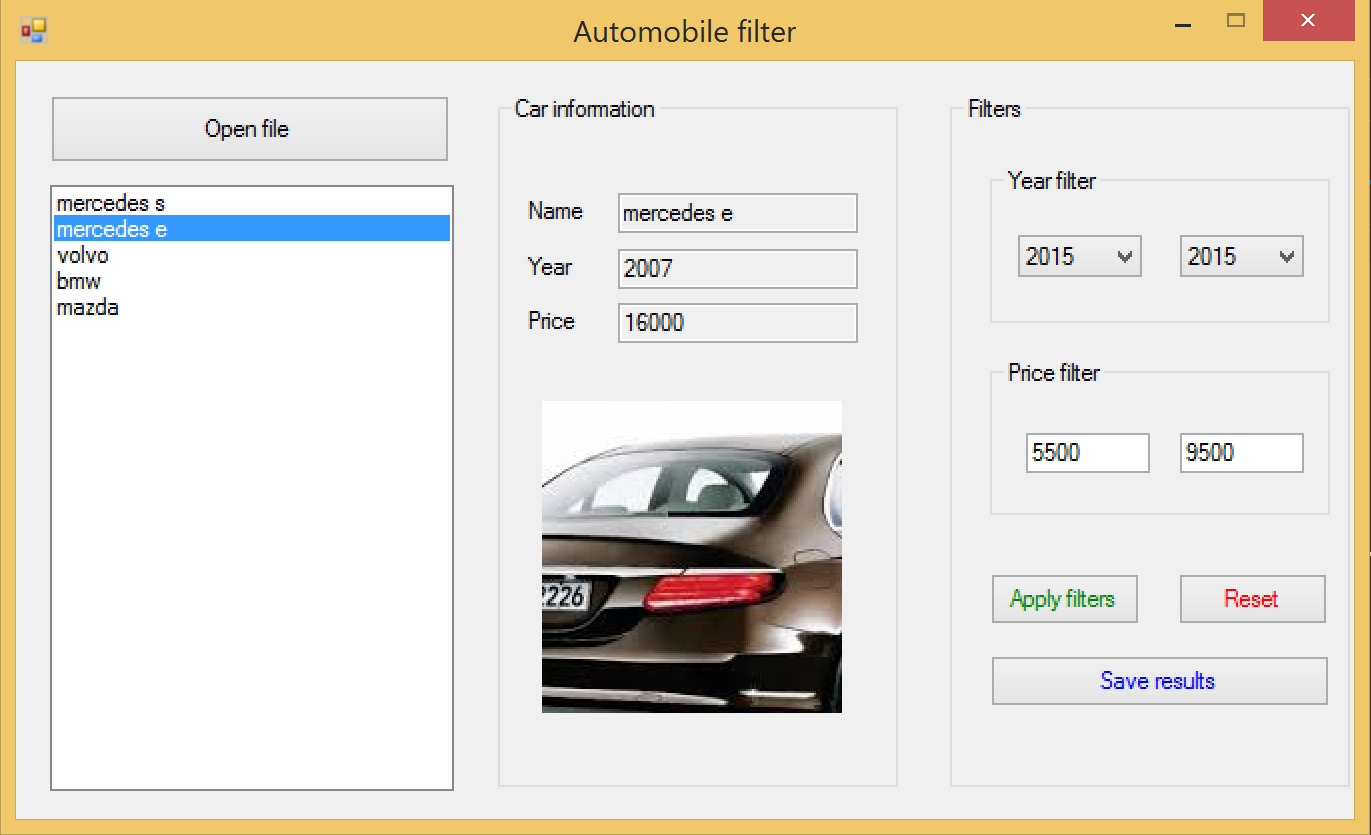
\includegraphics[width=150mm,height=90mm]{img/screen}
  \caption{Изображение итоговой формы}
  \label{fig:screen}
\end{figure}

Исходный текст разработанной программы расположен в приложении~А.

\newpage
